\chapter{Grundlagen der Mechanik}\label{ch:mech}
\section{Starrk\"orperbewegung}\label{sec:mech_starrkoerperbewegung}
Die Bewegung eines Punktes $p$ im euklidischen Raum wird durch die Angabe seiner Position in Bezug zu einem intertialen normierten Rechtssystem $\KOS{I}$ zu jedem Zeitpunkt $t$ eindeutig beschrieben. Die Position des Punktes $\vect{p}$ sei durch den Vektor $\left( x, y, z \right)^{T} \in \R^{3}$ gegeben. Die Trajektorie von $\vect{p}$ kann dann durch die parametrisierte Bahn $\vect{p}\of{t}=\left(x\of{t}, y\of{t}, z\of{t}\right) \in \R^{3} $ beschrieben werden. Da nicht die Bewegung von einzelnen Punkten, sondern die Bewegung eines Starrk\"orpers beschrieben werden soll, soll zun\"achst der Begriff Starrk\"orper definiert werden.

\begin{defn}[Starrk\"orper] Ein Starrk\"orper ist dadurch gekennzeichnet, dass die Distanz zweier beliebiger Punkte $\vect{p}, \vect{q}$, welche auf dem K\"orper liegen, unabh\"angig von der Bewegung des K\"orpers, immer konstant bleibt. Die anf\"angliche Position des Punktes $\vect{p}$ sei beschrieben durch $\vect{p}\of{0}$. Die Position nach einer beliebigen Zeit $t$ (und einer beliebigen Bewegung) sei beschrieben durch $\vect{p}\of{t}$. Die Nomenklatur gelte f\"ur den Punkt $\vect{q}$ analog. F\"ur einen Starrk\"orper wird gefordert: \begin{align*}
\norm{\vect{p}\of{t} - \vect{q}\of{t}}&=\norm{\vect{p}\of{0}-\vect{q}\of{0}} = \text{konstant}
\end{align*}
\end{defn}
Eine Starrk\"orperbewegung kann prinzipiell aus Rotation, Translation oder einer \"Uberlagerung dieser Bewegungen bestehen. Wird ein K\"orper durch eine Teilmenge $\set{O} \in \R^{3}$ beschrieben, so kann seine Bewegung als eine kontinuierliche Zuordnung $g\of{t}: \set{O} \to R^{3}$ beschrieben werden. Die kontinuierliche Zuordnungsvorschrift $g\of{t}$ beschreibt, wie sich die einzelnen Punkte des K\"orpers relativ zu einem inertialen, festen Koordinatensystem mit Voranschreiten der Zeit $t$ bewegen. Die Zuordnungsvorschrift $g$ darf dabei die Distanz zwischen Punkten des K\"orpers und die Orientierung von Vektoren, welche Punkte des K\"orpers verbinden, nicht ver\"andern. Damit ergibt sich die Definition einer Abbildung von Starrk\"orpern: 

\begin{defn}[Abbildung eines Starrk\"orpers] \cite{Murray1994} Eine Zuordnungsvorschrift $g: \R^{3} \to \R^{3}$ ist die Abbildung eines Starrk\"orpers genau dann, wenn sie folgende Eigenschaften besitzt: \begin{enumerate}
\item Distanzen bleiben unver\"andert: $\norm{g\of{\vect{p}}- g\of{\vect{q}}}=\norm{\vect{p}- \vect{q}}$ f\"ur alle Punkte $ \vect{p}, \vect{q} \in \R^{3}$
\item Das Kreuzprodukt bleibt erhalten: $g\of{\vect{v}\times \vect{w}} = g\of{\vect{v}}\times g\of{\vect{w}}$ f\"ur alle Vektoren $\vect{v}, \vect{w} \in \R^{3}$.
\end{enumerate}
\end{defn}

\begin{rem} Man kann mit Hilfe der Polarisationsformel zeigen, dass das Skalarprodukt durch die Abbildungsvorschrift $g$ f\"ur einen Starrk\"orper erhalten bleibt \cite{Murray1994}: \begin{align*}
\skalar{\vect{v}}{\vect{w}}&= \skalar{g\of{\vect{v}}}{g\of{\vect{w}}}.
\end{align*}
Ein orthonormales Rechtssystem wird durch die Abbildungsvorschrift $g$ demnach wieder in ein orthonormales Rechtssystem transformiert.
\end{rem}
Der Astronom und Mathematiker Giulio Mozzi zeigte bereits 1763, dass eine r\"aumliche Bewegung in eine Drehung und eine Verschiebung entlang der Drehachse zerlegt werden kann. Da sich die Teilchen eines Starrk\"orpers nicht relativ zueinander bewegen k\"onnen, kann die Bewegung eines Starrk\"orpers durch die relative Bewegung eines k\"orperfesten Koordinatensystems $\KOS{K}$ zu einem Inertialsystem $\KOS{I}$ beschrieben werden. Das Koordinatensystem $\KOS{K}$ erf\"ulle dabei die in Abschnitt \ref{sec:kos_rechtssys} genannten Eigenschaften. Das k\"orperfeste Koordinatensystem habe seinen Ursprung in einem beliebigen Punkt $Q$ des K\"orpers. Die Orientierung von $\KOS{K}$ beschreibt die Rotation des K\"orpers und die Lage des Ursprungs von $\KOS{K}$ relativ zum Inertialsystem beschreibt den translatorischen Anteil der Starrk\"orperbewegung. Der K\"orper ist in \figureref{fig:mech_starrkoerperbewegung_koerper} abgebildet. Hat $\KOS{K}$ die Einheitsvektoren $\vect{u}, \vect{w}, \vect{v}$, dann kann die Bewegung von $\KOS{K}$ durch die Abbildung $g$ beschrieben werden. Genauer gesagt liefert $g\of{\vect{u}}, g\of{\vect{w}}, g\of{\vect{v}}$ die Orientierung von $\KOS{K}$ und $g\of{\vect{p}}$ die Lage des Ursprungs nach einer Starrk\"orperbewegung. \newline
Beschreibt man die Orientierung eines Starrk\"orpers mit Hilfe eines Ortsvektors $\vect{\tensor*[_I]{q}{}}$, welcher auf den Ursprung $Q$ des k\"orperfesten Koordinatensystems zeigt, einem Ortsvektor $\vect{\tensor*[_I]{p}{}}$, welcher auf einen beliebigen Punkt $P$ des K\"orpers mit $\vect{\tensor*[_I]{q}{}} \neq \vect{\tensor*[_I]{p}{}}$ zeigt und dem Richtungsvektor $\vect{\tensor*[_I]{s}{}}$, welcher die Punkte $Q$ und $P$ verbindet, dann erh\"alt man mit folgender Rechnung eine Formel zur Beschreibung der Bewegung in homogenen Koordinaten. \hfill \newline
Die Vektoren $\vectHomog{\tensor*[_I]{s}{}}$ und $\vectHomog{\tensor*[_K]{p}{}}$ beschreiben offensichtlich den gleichen k\"orperfesten Punkt $P$. Im ersten Fall in Relation zum Inertialsystem und im zweiten Fall relativ zum k\"orperfesten System. Es gilt \begin{align*}
\vectHomog{\tensor*[_I]{s}{}}&=\vectHomog{\tensor*[_K]{p}{}}. 
\end{align*}
\begin{figure}[htb]
\begin{center}
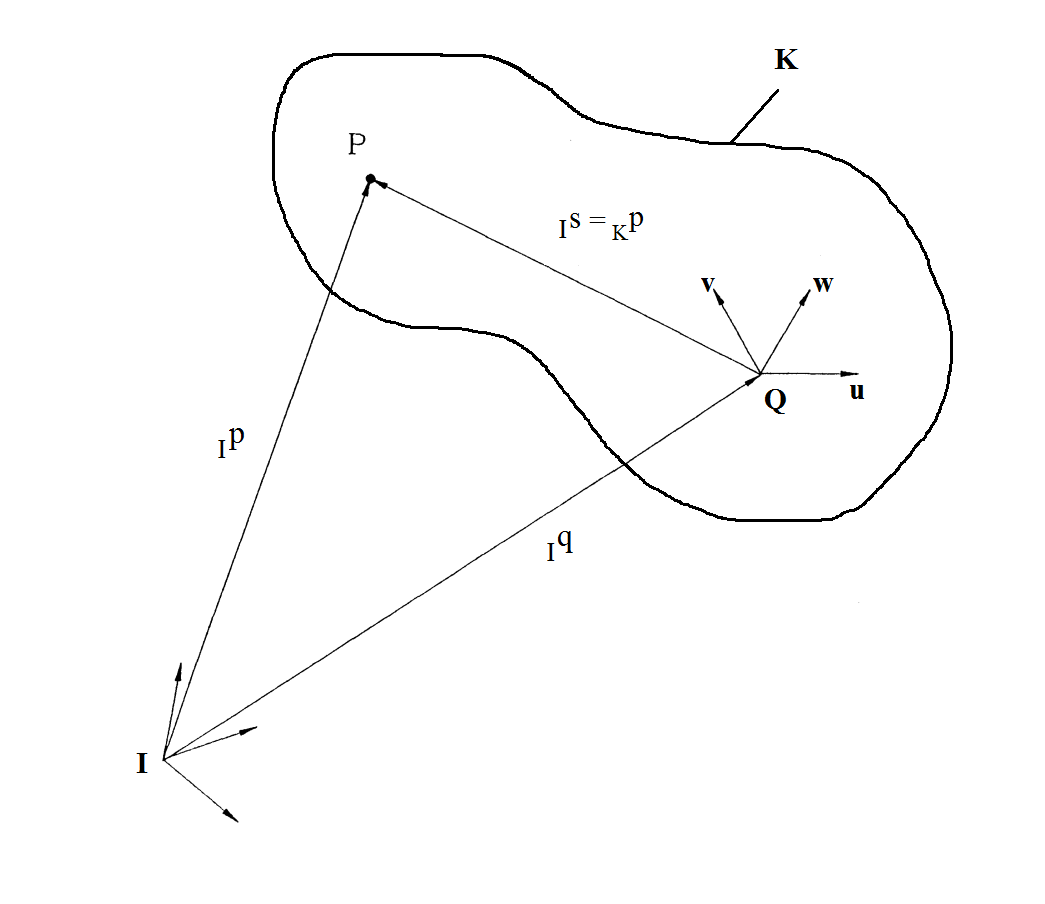
\includegraphics[width=0.75\textwidth]{abbildungen/04_koerperBwg.png}
\caption{Starrk\"orper mit k\"orperfestem Koordinatensystem}
\label{fig:mech_starrkoerperbewegung_koerper}
\end{center}
\end{figure}

\begin{rem}[Addition von Vektoren mit verschiedenen Basen] Die Vektoren $\vectHomog{\tensor*[_I]{s}{}}, \vectHomog{\tensor*[_K]{p}{}}$ beschreiben grafisch den gleichen Vektor. Die Vektoren sind bez\"uglich unterschiedlicher Basen definiert. Die jeweilige Basis sind die Einheitsvektoren vom Koordinatensystem $\KOS{I}$ beziehungsweise $\KOS{K}$. Die numerischen Komponenten dieser Vektoren sind also verschieden. Eine Addition von Vektoren mit unterschiedlichen Basen ist nicht m\"oglich. Statt dessen muss einer der Vektoren vor der Addition in die Basis des anderen Vektors transformiert werden. Die Rechnung \begin{align*}
\vect{\tensor*[_I]{p}{}}&= \vect{\tensor*[_I]{q}{}}+ \vect{\tensor*[_I]{s}{}}
\end{align*} ist legitim, die Rechnung \begin{align*}
\vect{\tensor*[_I]{p}{}}&= \vect{\tensor*[_I]{q}{}}+ \vect{\tensor*[_K]{p}{}}
\end{align*} hingegen nicht. 
\end{rem}

Es gilt nach \eqnref{gl:kos_transfHomog_transf_punktTransfo} f\"ur die Transformation des Punktes $P$ von k\"orpefesten Koordinaten in das Inertialsystem\begin{align}
\vectHomog{\tensor*[_I]{p}{}}&= \tensor*[^K_I]{\matr{T}}{} \vectHomog{\tensor*[_K]{p}{}} \label{gl:mech_starrkoerperbewegung_ansatz} \\ 
\begin{bmatrix} \vect{\tensor*[_I]{p}{}} \\ 1 \end{bmatrix}&= \begin{bmatrix}
\tensor*[^K_I]{\matr{R}}{} & \vect{\tensor*[_I]{q}{}} \\ \vect{0} & 1 \end{bmatrix} \begin{bmatrix}
\vect{\tensor*[_K]{p}{}} \\ 1 \end{bmatrix} \nonumber
\end{align}
Zur besseren Unterscheidbarkeit soll die Zeitabh\"angigkeit jetzt explizit angegeben werden. Nach der Starrk\"orperbedingung ist $\vectHomog{\tensor*[_K]{p}{}}$ konstant, die Elemente der Transformationsmatrix $\tensor*[^K_I]{T}{}$ sind hingegen nicht zwangsl\"aufig unabh\"angig von der Zeit. Differenziert man \eqnref{gl:mech_starrkoerperbewegung_ansatz} nach der Zeit, so folgt daher \begin{align*}
\frac{\td}{\td t}\of{\vectHomog{\tensor*[_I]{p}{}}\of{t}}&= \frac{\td }{\td t}\of{\tensor*[^K_I]{\matr{T}}{}\of{t} \vectHomog{\tensor*[_K]{p}{}}}
\intertext{mit der Produktregel folgt dann}
\frac{\td}{\td t}\of{\vectHomog{\tensor*[_I]{p}{}}\of{t}}&= \frac{\td }{\td t}\of{\tensor*[^K_I]{\matr{T}}{}\of{t}} \vectHomog{\tensor*[_K]{p}{}} + \tensor*[^K_I]{\matr{T}}{}\of{t}\com{\frac{\td }{\td t}\of{\vectHomog{\tensor*[_K]{p}{}}}}{$=0$}
\intertext{und mit \eqnref{gl:kos_transfHomog_homKoord_ableitung}}
\begin{bmatrix} \vect{\tensor*[_I]{\dot{p}}{}}\of{t} \\ 0 \end{bmatrix}&= \begin{bmatrix}
\tensor*[^K_I]{\dot{\matr{R}}}{}\of{t} & \vect{\tensor*[_I]{\dot{q}}{}}\of{t} \\ \vect{0} & 0 \end{bmatrix} \begin{bmatrix}
\vect{\tensor*[_K]{p}{}} \\ 1 \end{bmatrix}.
\end{align*}
Der so erhaltene Geschwindigkeitsterm hat den Nachteil, dass sich die Gleichungselemente auf verschiedene Bezugssysteme beziehen. Daher transformiert man den Vektor des Punktes $P$ wieder in das Inertialsystem und erh\"alt damit die kompakte Form der Bewegungsgleichung in homogenen Koordinaten \begin{align}
\begin{bmatrix} \vect{\tensor*[_I]{\dot{p}}{}}\of{t} \\ 0 \end{bmatrix}&= \tensor*[^K_I]{\dot{T}}{} \inv{\tensor*[^K_I]{T}{}}\of{t} \begin{bmatrix}
\vect{\tensor*[_I]{p}{}}\of{t} \\ 1 \end{bmatrix} \nonumber \\ 
\vectHomog{\tensor*[_I]{\dot{p}}{}}\of{t}&= \tensor*[^K_I]{\dot{T}}{} \inv{\tensor*[^K_I]{T}{}}\of{t} \vectHomog{\tensor*[_I]{p}{}}\of{t} \label{gl:mech_starrkoerperbewegung_bwgGlHomoKompakt}
\end{align}

Notiert man \eqnref{gl:mech_starrkoerperbewegung_bwgGlHomoKompakt} ausf\"uhrlich, so kann man eine Matrix $\matr{\Omega}$ nach Abschnitt \ref{sssec:kos_transfHomog_rots_eigensch} einf\"uhren, welche die Komponenten des Winkelgeschwindigkeitsvektors enth\"alt. Es folgt unter Verwendung von \eqnref{gl:kos_transfHomog_homKoord_transfoInv} f\"ur \eqnref{gl:mech_starrkoerperbewegung_bwgGlHomoKompakt}
\begin{align*}
\begin{bmatrix} \vect{\tensor*[_I]{\dot{p}}{}}\of{t} \\ 0 \end{bmatrix}&= \begin{bmatrix}
\tensor*[^K_I]{\dot{\matr{R}}}{}\of{t} & \vect{\tensor*[_I]{\dot{q}}{}}\of{t} \\ \vect{0} & 0 \end{bmatrix} \begin{bmatrix}
\transp{\tensor*[^K_I]{\matr{R}}{}}\of{t} & -\transp{\tensor*[^K_I]{\matr{R}}{}}\of{t} \vect{\tensor*[_I]{q}{}}\of{t} \\ \vect{0} & 1 \end{bmatrix} \begin{bmatrix}
\vect{\tensor*[_I]{p}{}}\of{t} \\ 1 \end{bmatrix} 
\\
\begin{bmatrix} \vect{\tensor*[_I]{\dot{p}}{}}\of{t} \\ 0 \end{bmatrix}&= 
\begin{bmatrix}
\tensor*[^K_I]{\dot{\matr{R}}}{}\of{t} \transp{\tensor*[^K_I]{\matr{R}}{}}\of{t} & -\tensor*[^K_I]{\dot{\matr{R}}}{}\of{t} \transp{\tensor*[^K_I]{\matr{R}}{}}\of{t}\vect{\tensor*[_I]{q}{}}\of{t} + \vect{\tensor*[_I]{\dot{q}}{}}\of{t} \\ 
\vect{0} & 0
\end{bmatrix} 
\begin{bmatrix}
\vect{\tensor*[_I]{p}{}}\of{t} \\ 1
\end{bmatrix}
\end{align*}
Setzt man jetzt \begin{align}
\tensor*[_I]{\matr{\Omega}}{}\of{t}&= \tensor*[^K_I]{\dot{\matr{R}}}{}\of{t} \transp{\tensor*[^K_I]{\matr{R}}{}}\of{t} \label{gl:mech_starrkoerperbewegung_winkelGeschwMatr}
\end{align} in obigen Ausdruck ein, so erh\"alt man die ausf\"uhrliche Darstellung der Bewegungsgleichung in homogenen Koordinaten zu 
\begin{align}
\begin{bmatrix} \vect{\tensor*[_I]{\dot{p}}{}}\of{t} \\ 0 \end{bmatrix}&= 
\begin{bmatrix}
\tensor*[_I]{\matr{\Omega}}{}\of{t} & -\tensor*[_I]{\matr{\Omega}}{}\of{t}\vect{\tensor*[_I]{q}{}}\of{t} + \vect{\tensor*[_I]{\dot{q}}{}}\of{t} \\ 
\vect{0} & 0
\end{bmatrix} 
\begin{bmatrix}
\vect{\tensor*[_I]{p}{}}\of{t} \\ 1
\end{bmatrix}. \label{gl:mech_starrkoerperbewegung_bwgGlHomoAusfue}
\end{align}
F\"uhrt man noch eine Enthomogenisierung von \eqnref{gl:mech_starrkoerperbewegung_bwgGlHomoAusfue} durch, so folgt ein Ausdruck f\"ur die Geschwindigkeit des K\"orperpunktes $P$ in kartesischen Koordinaten.
\begin{align}
\vect{\tensor*[_I]{\dot{p}}{}}\of{t}&= 
\tensor*[_I]{\matr{\Omega}}{}\of{t} \com{\left(
\vect{\tensor*[_I]{p}{}}\of{t} - 
\vect{\tensor*[_I]{q}{}}\of{t} \right)}{$=\vect{\tensor*[_I]{s}{}}\of{t}$} +
\vect{\tensor*[_I]{\dot{q}}{}}\of{t} 
\nonumber \\
\vect{\tensor*[_I]{\dot{p}}{}}\of{t}&= \vect{\tensor*[_I]{\dot{q}}{}}\of{t} + 
\tensor*[_I]{\matr{\Omega}}{}\of{t} \vect{\tensor*[_I]{s}{}}\of{t} \label{gl:mech_starrkoerperbewegung_bwgGlKart}
\end{align}
Die \eqnref{gl:mech_starrkoerperbewegung_bwgGlKart} kann ohne den Umweg \"uber homogene Koordinaten direkt hergeleitet werden. Dazu geht man erneut von einem Starrk\"orper mit den festen Punkten $Q, P$, den zugeh\"origen Ortsvektoren $\vect{\tensor*[_I]{q}{}}, \vect{\tensor*[_I]{p}{}}$ und dem Verbindungsvektor $\vect{\tensor*[_I]{s}{}}$ der zwei K\"orperpunkte aus. Als Ausgangsgleichung dient die Summengleichung dieser drei Vektoren. \begin{align*}
\vect{\tensor*[_I]{p}{}}\of{t}&=\vect{\tensor*[_I]{q}{}}\of{t} + \vect{\tensor*[_I]{s}{}}\of{t}
\intertext{Die Differentiation nach der Zeit liefert}
\ddt{}\left(\vect{\tensor*[_I]{p}{}}\of{t}\right)&=\ddt{}\left(\vect{\tensor*[_I]{q}{}}\of{t}\right) + \ddt{}\left(\vect{\tensor*[_I]{s}{}}\of{t}\right)
\intertext{woraus unter Beachtung der Starrk\"orperbedingung}
\norm{\vect{\tensor*[_I]{p}{}}\of{t} - \vect{\tensor*[_I]{q}{}}\of{t}} &\equiv \norm{\vect{\tensor*[_I]{s}{}}\of{t}} = konstant \\
\implies \skalar{\vect{\tensor*[_I]{s}{}}\of{t}}{\vect{\tensor*[_I]{s}{}}\of{t}}&= konstant
\intertext{folgt}
\ddt{}\left(\skalar{\vect{\tensor*[_I]{s}{}}\of{t}}{\vect{\tensor*[_I]{s}{}}\of{t}}\right) &=0.
\end{align*}
Die Anwendung der Produktregel liefert %(siehe Bspw. \cite[S.20]{Mathiak2015})
\begin{align*}
\ddt{}\left(\skalar{\vect{\tensor*[_I]{s}{}}\of{t}}{\vect{\tensor*[_I]{s}{}}\of{t}}\right) &=0 \\
\skalar{\vect{\tensor*[_I]{\dot{s}}{}}\of{t}}{\vect{\tensor*[_I]{s}{}}\of{t}} + \skalar{\vect{\tensor*[_I]{s}{}}\of{t}}{\vect{\tensor*[_I]{\dot{s}}{}}\of{t}}&=0,
\intertext{was sich durch die Kommutativit\"at des Skalarprodukts zusammenfassen l\"asst zu}
2 \skalar{\vect{\tensor*[_I]{\dot{s}}{}}\of{t}}{\vect{\tensor*[_I]{s}{}}\of{t}}&= 0. 
\end{align*}
Nach der in Kapitel \ref{ch:mathGrundl} aufgef\"uhrten Bemerkung \ref{rem:mathGrundl_punkteVektoren_skalarProd_ortho} impliziert diese Gleichung, dass
\begin{align*}
\vect{\tensor*[_I]{s}{}}\of{t} &\perp \vect{\tensor*[_I]{\dot{s}}{}}\of{t}
\end{align*}
gilt. Da der Geschwindigkeitsvektor $\vect{\tensor*[_I]{\dot{s}}{}}\of{t}$ senkrecht auf $\vect{\tensor*[_I]{s}{}}\of{t}$ stehen soll ist es sinnvoll einen Vektor $\vect{\tensor*[_I]{\omega}{}}\of{t}=\left( \omega_{x} , \omega_{y} , \omega_{z} \right)^{T}$ wie folgt einzuf\"uhren: \begin{align*}
\vect{\tensor*[_I]{\dot{s}}{}}\of{t} &= \vect{\tensor*[_I]{\omega}{}}\of{t} \times \vect{\tensor*[_I]{s}{}}\of{t}
\end{align*}
Damit berechnet sich die Geschwindigkeit eines beliebigen Punktes des K\"orpers zu: \begin{align}
\ddt{}\left(\vect{\tensor*[_I]{p}{}}\of{t}\right)&= \vect{\tensor*[_I]{\dot{p}}{}}\of{t} =\vect{\tensor*[_I]{\dot{q}}{}}\of{t}  + \vect{\tensor*[_I]{\omega}{}}\of{t} \times \vect{\tensor*[_I]{s}{}}\of{t} \label{gl:starrKAllgGeschw}
\end{align}
Ersetzt man den Term $\vect{\tensor*[_I]{\omega}{}}\of{t} \times$ durch eine Multiplikation mit einer schiefsymmetrischen Matrix $\tensor*[_I]{\matr{\Omega}}{}=\begin{bmatrix}
0& -\omega_{z} & \omega_{y}\\ \omega_{z}& 0 &-\omega_{x} \\ -\omega_{y} & \omega_{x} & 0
\end{bmatrix}$ nach \eqnref{gl:SdT_mathGrundl_punkteVektoren_kreuzProdMatrix}, so erh\"alt man den Ausdruck \begin{align}
\vect{\tensor*[_I]{\dot{p}}{}}\of{t} &= \vect{\tensor*[_I]{\dot{q}}{}}\of{t} + \tensor*[_I]{\matr{\Omega}}{} \vect{\tensor*[_I]{s}{}}\of{t},
\end{align} was \eqnref{gl:mech_starrkoerperbewegung_bwgGlKart} entspricht. Diese Variante der Herleitung f\"ur die Bewegungsgleichung eines Starrk\"orpers ist also \"aquivalent zu der Herleitung mit Hilfe homogener Transformationsmatrizen. 

%\subsection{Vektor der Winkelgeschwindigkeit}
%\begin{align*}
%\matr{\Omega}&= \dot{\matr{R}} \transp{\matr{R}} \\
%&= \begin{pmatrix}
%{ \dot{r}_{11}}&{ \dot{r}_{12}}&{ \dot{r}_{13}}\\
% { \dot{r}_{21}}&{ \dot{r}_{22}}&{ \dot{r}_{23}}\\
% { \dot{r}_{31}}&{ \dot{r}_{32}}&{ \dot{r}_{33}}
%\end{pmatrix} \begin{pmatrix}
% { r_{11}}&{ r_{12}}&{ r_{13}}\\
% { r_{21}}&{ r_{22}}&{ r_{23}}\\
% { r_{31}}&{ r_{32}}&{ r_{33}}
%\end{pmatrix}^{T} \\
%&= \begin{pmatrix}
%\dot{r}_{11}\,r_{11}+\dot{r}_{12}\,r_{12}+\dot{r}_{13}\,r_{13}&\dot{r}_{11}\,r_{21}+\dot{r}_{12}\,r_{22}+\dot{r}_{13}\,r_{23}&\dot{r}_{11}\,r_{31}+\dot{r}_{12}\,r_{32}+\dot{r}_{13}\,r_{33}\\
%\dot{r}_{21}\,r_{11}+\dot{r}_{22}\,r_{12}+\dot{r}_{23}\,r_{13}&\dot{r}_{21}\,r_{21}+\dot{r}_{22}\,r_{22}+\dot{r}_{23}\,r_{23}&\dot{r}_{21}\,r_{31}+\dot{r}_{22}\,r_{32}+\dot{r}_{23}\,r_{33}\\
%\dot{r}_{31}\,r_{11}+\dot{r}_{32}\,r_{12}+\dot{r}_{33}\,r_{13}&\dot{r}_{31}\,r_{21}+\dot{r}_{32}\,r_{22}+\dot{r}_{33}\,r_{23}&\dot{r}_{31}\,r_{31}+\dot{r}_{32}\,r_{32}+\dot{r}_{33}\,r_{33}
%\end{pmatrix} \\
%&= \begin{pmatrix}
%0 & -\omega_3 & \omega_2\\
%\omega_3 & 0 & -\omega_1\\
%-\omega_2 & \omega_1 & 0
%\end{pmatrix} \\
%\vect{\omega}&= \begin{pmatrix}
%\omega_1 \\ \omega_2 \\ \omega_3
%\end{pmatrix}\\
%&= \begin{pmatrix}
%\dot{r}_{31}\,r_{21}+\dot{r}_{32}\,r_{22}+\dot{r}_{33}\,r_{23} \\
%\dot{r}_{11}\,r_{31}+\dot{r}_{12}\,r_{32}+\dot{r}_{13}\,r_{33} \\
%\dot{r}_{21}\,r_{11}+\dot{r}_{22}\,r_{12}+\dot{r}_{23}\,r_{13}
%\end{pmatrix} \\
%&= \begin{pmatrix}
%\skalar{\dot{v}}{w}\\
%\skalar{\dot{u}}{v}\\
%\skalar{\dot{w}}{u}
%\end{pmatrix}
%\end{align*}
%\begin{align*}
%\intertext{Drall}
%\matr{L}_{P}&=\begin{pmatrix}
%A \omega_{x}  -F \omega_{y}  -E \omega_{z} \\
%-F \omega_{x}  +B \omega_{y}  -D \omega_{z} \\
%-E \omega_{x}  -D \omega_{y}  +C \omega_{z}
%\end{pmatrix} \\
%\end{align*}
%\begin{align*}
%\intertext{Tr\"agheitstensor}
%\matr{L}_{P}&=\matr{J}_{P} \vect{\omega} \\
%\matr{J}_{P}&=\begin{pmatrix}
%A  & -F  & -E  \\
%-F  & B  & -D  \\
%-E  & -D  & C 
%\end{pmatrix} \\
%\frac{1}{2} \vect{\omega}\matr{L}_{P} &= \frac{1}{2}( \dots \\
% &\quad \omega_{x} ( A\omega_{x}-E\omega_{z}- F\omega_{y} ) + \dots \\
% &\quad \omega_{y} ( B\omega_{y}-  D \omega_{z}-F\omega_{x} ) + \dots \\
% &\quad \omega_{z} ( C\omega_{ z}-  D \omega_{y}-E\omega_{x} ))
%\intertext{Einsetzen der Terme f\"ur Komponenten der Winkelgeschw.}
% &=\frac{1}{2}\left( A(\dot{v}^2)(w^2) + B(\dot{u}^2)(v^2)+C(\dot{w}^2)(u^2)\right)+ \dots \\
% &\quad \frac{1}{2}\left( -D\dot{u}\dot{w}\com{u v}{=0}  -E\dot{v}\dot{w}\com{u w}{=0} - F\dot{u}\dot{v}\com{v w}{=0} \right)
%\end{align*}
\section{Lagrange Gleichung 2. Art}\label{sec:mech_lag2}
Der Ansatz nach Lagrange ist eine M\"oglichkeit, um die Bewegung von Systemen mit Zwangsbedingungen zu beschreiben. Ein fr\"uhes Werk zur Arbeit mit diesem Ansatz wurde von N. W. Akimoff \cite{Akimoff1917} verfasst. Eine \"Ubersicht \"uber weitere Formalismen zur Beschreibung von Mehrk\"orpersystemen ist im Werk von W. Schiehlen und P. Eberhard \cite[S. 131 ff.]{Schiehlen2014} zu finden. Im Buch von Pfeiffer \cite[S.56 ff.]{Pfeiffer2014} wird die Eignung verschiedener Verfahren bewertet. Im Rahmen dieser Arbeit wird nur der Ansatz von Lagrange behandelt. Ein besonderes Augenmerk liegt dabei auf der Darstellung der bekannten Gleichungen in den generalisierten Koordinaten, welche man bei Parametrierung eines Mehrk\"orpersystems mit nat\"urlichen Koordinaten erh\"alt. Das Ziel ist eine ausf\"uhrliche Herleitung der Ansatzgleichungen, wie sie in der Arbeit von V. Cossalter und R. Lot in \cite{Cossalter2002} verwendet werden. \hfill \newline 
%\subsection{Erg\"anzungen}
%\cite[S.38]{Bestle2012}, \cite[S.90]{GeorgRill2014}, \cite[S.87]{Schramm2010}, \hfill \newline
%Lagrange sollte man nicht verwenden. Dies bedeutet, dass die direkte Auswertung der Lagrangeschen Gleichungen zweiter Art in ihrer ursprünglichen Form (4.61) auf
%einen unnötigen Rechenaufwand führt. Bei der Aufstellung der Bewegungsgleichungen nach
%dem d’Alembertschen Prinzip kommt man dagegen unmittelbar ans Ziel. Deshalb wird in den
%nächsten Kapiteln nur noch das d’Alembertsche bzw. das Jourdainsche Prinzip herangezogen.
%Diesen beiden Prinzipien liegt aber letztlich die Aufteilung des Raumes, der von den Koordinaten eines freigeschnittenen mechanischen Systems aufgespannt wird, in zwei orthogonale
%Unterräume für die freien bzw. gesperrten Bewegungsrichtungen zugrunde. Diese orthogonalen
%Unterräume sind unter der Voraussetzung idealer Kräfte, wie sie z. B. in gewöhnlichen Mehrkörpersystemen auftreten, voneinander unabhängig, was auf ungekoppelte Bewegungs- und Reaktionsgleichungen führt. \cite[S. 96]{Schiehlen2014}  \hfill \newline

%\cite[S.42]{Pfeiffer2014} -> das k\"onnte wirklich noch mal helfen \hfill \newline
%\subsection{Richtiger Inhalt}
%\paragraph{Hier fehl ein einf\"uhrungssatz, wo lagrange her kommt}
Gegeben sei ein System, welches durch $n$ generalisierten Koordinaten $\vect{q}= \transp{\of{ q_{1}, q_{2}, \dots,   q_{n}}} $, welche nicht notwendigerweise voneinander unabh\"angig sein m\"ussen, und $m$ holonomen \footnote{Holonome Zwangsbedingungen sind solche, die von der Position aber nicht von der Geschwindigkeit eines K\"orpers abh\"angen.} Zwangsbedingungen $\vect{\phi}=\transp{\of{\phi_{1} , \phi_{2} , \dots , \phi_{m}}}=\vect{0}$ charakterisiert wird. Die kinetische Energie $T$ und potentielle Energie $V$ sei durch $L=T-V$ verkn\"upft. Das gesamte System l\"asst sich nach \cite[S. 124]{Jalon1994} dann mit der \textit{Gleichung von Lagrange 2. Art} beschreiben, welche in \eqnref{gl:mech_lagrange2ArtDefAllg} angegeben ist.
\begin{align}
\int_{t_{1}}^{t_{2}}\left[ \com{\delta\transp{\vect{q}}}{$h\of{t}$} \com{\left(  \ddt{}\of{\frac{\d L}{\d \dot{\vect{q}}}} - \frac{\d L}{\d \vect{q}} + \transp{\matr{\Phi}}_{\vect{q}} \vect{\lambda} - \vect{Q}_{ex} \right)}{$g\of{t}$} \right] \td t &=\vect{0}, \label{gl:mech_lagrange2ArtDefAllg} 
\end{align} 
wobei die Matrix $\matr{\Phi}_{\vect{q}}$ die Jacobi-Matrix der Zwangsbedingungen bez\"uglich der generalisieren Koordinaten ist und $\vect{\lambda}$ hat die Lagrange-Multiplikatoren als Komponenten. 
Es gelten die Dimensionen
\begin{align*} 
\delta \vect{q}&\in\R^{n} &L&\in \R &\vect{q}&\in \R^{n} &\matr{\Phi}_{\vect{q}}&\in \R^{m \times n} &\vect{\lambda}&\in \R^{m} &\vect{Q}_{ex}&\in R^{n}
\end{align*}
Mit Hilfe des Fundamentallemmas der Variationsrechnung \cite[S. 107 f.]{Reddy2002} l\"asst sich \eqnref{gl:mech_lagrange2ArtDefAllg} umformen. Das Fundamentallemma der Variationsrechnung kann  wie folgt formuliert werden: \hfill \newline
Eine integrierbare Funktion $g\of{t}$ entspricht der Nullfunktion auf dem abgeschlossenen Intervall $[a, b]$, wenn die Aussage \begin{align*}
\int_{a}^{b} g\of{t}\cdot h\of{t} \td t &=0
\end{align*}
f\"ur beliebige stetige Funktionen $h\of{t}$ in diesem Intervall erf\"ullt ist. \hfill \newline 
F\"ur beliebige Variationen des Ortes $h\of{t}=\delta \transp{\vect{q}\of{t}}$ soll  \eqnref{gl:mech_lagrange2ArtDefAllg} erf\"ullt sein und damit ist $g\of{t}$ gleich der Nullfunktion. Die $m$ Langrange-Multiplikatoren $\lambda$ sind daher so zu w\"ahlen, dass 
 \begin{align}
  \ddt{}\of{\frac{\d L}{\d \dot{\vect{q}}}} - \frac{\d L}{\d \vect{q}} + \transp{\matr{\Phi}}_{q} \vect{\lambda} - \vect{Q}_{ex} &=\vect{0} \label{gl:mech_lagrange2ArtDef}
\end{align}
gilt. Beachtet man nun, dass die Potentialkr\"afte $V$ wie in \cite[S. 190]{J.L.Humar2002} angegeben wird, nicht von den Geschwindigkeiten $\dot{\vect{q}}$ abh\"angen, so kann man \eqnref{gl:mech_lagrange2ArtDef} derart umformen, dass die generalisierten Kr\"afte $\vect{Q}$, welche sich aus der virtuellen Arbeit ergeben, explizit auftreten. \begin{align}
\ddt{}\of{\frac{\d (T-V)}{\d \dot{\vect{q}}}} - \frac{\d (T-V)}{\d \vect{q}} + \transp{\matr{\Phi}}_{q} \vect{\lambda} - \vect{Q}_{ex} &=\vect{0} \nonumber \\
\ddt{}\of{\frac{\d T}{\d \dot{\vect{q}}}} - \frac{\d T}{\d \vect{q}} + \frac{\d V}{\d \vect{q}}+ \transp{\matr{\Phi}}_{q} \vect{\lambda} - \vect{Q}_{ex} &=\vect{0} \nonumber \\
\ddt{}\of{\frac{\d T}{\d \dot{\vect{q}}}} - \frac{\d T}{\d \vect{q}} + \transp{\matr{\Phi}}_{q} \vect{\lambda} - \vect{Q} &=\vect{0} \label{gl:mech_lagrange2ArtDefCossalter}
\end{align}
Diese Gleichung der Dimension $n$ bildet gemeinsam mit den $m$ Zwangsbedingungen $\vect{\phi}=\vect{0}$ ein System von $\left( n + m\right)$ \acp{dae}. \hfill \newline
Lassen sich die Zwangsbedingungen derart umformen, dass die generalisierten Koordinaten $\vect{q}$ auf einen Satz von Minimalkoordinaten $\vect{q}_{min}\in R^{n-m}$ umformbar sind und k\"onnen au\ss{}erdem alle generalisierten Kr\"afte durch Ableitung der potentiellen Energie $V$ beschrieben werden,  so vereinfacht sich \eqnref{gl:mech_lagrange2ArtDef} zu
\begin{align}
\ddt{}\of{\frac{\d L}{\d \dot{\vect{q}}_{min}}} - \frac{\d L}{\d \vect{q}_{min}} &=0 \label{gl:lagrange2ArtDefMin} 
\end{align}
Die Umformung auf Minimalkoordinaten f\"uhrt aber zu sehr komplexen Darstellungen der Elemente von $\vect{q}_{min}$. Au\ss{}erdem ist die Umformung auf Minimalkoordinaten bei komplexen Systemen eine nicht triviale Aufgabe, da nicht offensichtlich ist, welche Elemente von $\vect{q}$ \"uberhaupt einen Satz von linear unabh\"angigen Koordinaten bilden k\"onnen. Werden Systeme mit nat\"urlichen Koordinaten nach Abschnitt \ref{sec:kos_natKoord} parametriert, so ist die Anzahl der generalisierten Koordinaten besonders hoch. Eine Systembeschreibung nach \eqnref{gl:mech_lagrange2ArtDefCossalter} ist daher zu bevorzugen. Im Folgenden wird daher auf die L\"osung dieser Gleichung eingegangen. 
  \subsection{Kinetische Energie}\label{ssec:mech_lag2_kinEn}
  Die kinetische Energie $K$ eines Starrk\"orpers wird durch die Geschwindigkeit eines beliebigen Punktes $P$ mit dem Ortsvektor $\vect{p}$, welcher ein Element des K\"orpers ist, und seiner Massenverteilung nach \eqnref{gl:kinEnergieAllgDef} beschrieben. Besteht ein System aus mehreren Teilk\"orpern, so wird \eqnref{gl:kinEnergieAllgDef} f\"ur jeden K\"orper einzeln betrachet. \cite[S. 206 ff.]{KurtMagnus2005} \begin{align}
  K&=\frac{1}{2} \int_{m} \dot{\vect{p}}^{2} \td m \label{gl:kinEnergieAllgDef}
  \end{align} Der Punkt $\vect{p}$ kann in den Koordinaten des k\"orperfesten Koordinatensystems angegeben werden. Dazu sind der Ursprung $\vect{q}$ und die Orientierung des k\"orperfesten Systems $\KOS{K}$ notwendig. Die Orientierung wird durch die Rotationsmatrix $\matr{R}$ nach \eqnref{gl:kos_transfHomog_rots_rotMatrDef} angegeben. Die Transformation von k\"orperfesten in inertiale Koordinaten geschieht dann nach \eqnref{gl:kos_transfHomog_transf_punktTransfo} mit Hilfe der von der Zeit abh\"angigen Transformationsmatrix \begin{align*}
  {T}\of{t}=\begin{bmatrix}  \matr{R}\of{t} & \vect{q}\of{t}\\ \vect{0} & 1 \end{bmatrix}.
  \end{align*} Die Zeitabh\"angigkeit wird im Folgenden nicht mehr explizit angegeben.\hfill \newline
 Seien die Koordinaten von $\vect{p}$ im Koordinatensystem $\KOS{K}$ in homogener Darstellung gegeben mit $\vect{\tensor*[_K]{p}{}}=\left(x, y, z, 1\right)^{T}$, so l\"asst sich die Bestimmungsgleichung der kinetischen Energie wie folgt umformen: \begin{align*}
  K&= \frac{1}{2}\int_{m} \left(\frac{\td}{\td t}\of{ \matr{T} \vect{\tensor*[_K]{p}{}}}\right)^{2} \td m
  \intertext{unter der Beachtung, dass $\vect{\tensor*[_K]{p}{}}$ zeitlich konstant ist, folgt}
  K &= \frac{1}{2}\int_{m} \of{x, y, z, 1} \transp{\dot{\matr{T}}} \dot{\matr{T}} \transp{\of{x, y, ,z, 1}} \td m
   \\
  &= \frac{1}{2}\int_{m} \of{x, y, z, 1} \begin{bmatrix}
  \dot{\vect{u}}^{2} & \skalar{{\dot{\vect{u}}}}{\dot{\vect{w}}} & \skalar{{\dot{\vect{u}}}}{\dot{\vect{v}}} & \skalar{{\dot{\vect{u}}}}{\dot{\vect{q}}} \\
   \skalar{{\dot{\vect{w}}}}{\dot{\vect{u}}} & \dot{\vect{w}}^{2} & \skalar{{\dot{\vect{w}}}}{\dot{\vect{v}}} & \skalar{{\dot{\vect{w}}}}{\dot{\vect{q}}} \\
   \skalar{{\dot{\vect{v}}}}{\dot{\vect{u}}} & \skalar{{\dot{\vect{v}}}}{\dot{\vect{w}}} & \dot{\vect{v}}^{2} & \skalar{{\dot{\vect{v}}}}{\dot{\vect{q}}} \\
   \skalar{{\dot{\vect{q}}}}{\dot{\vect{u}}} & \skalar{{\dot{\vect{q}}}}{\dot{\vect{w}}} & \skalar{{\dot{\vect{q}}}}{\dot{\vect{v}}} & \dot{\vect{q}}^{2} 
\end{bmatrix}   \transp{\of{x, y, z, 1}} \td m
\\
&= \frac{1}{2} \dot{\vect{q}}^{2} \int_{m} \td m + 
\frac{1}{2} \dot{\vect{u}}^{2} \int_{m} x^{2} \td m + 
\frac{1}{2} \dot{\vect{w}}^{2} \int_{m} y^{2} \td m + 
\frac{1}{2} \dot{\vect{v}}^{2} \int_{m} z^{2} \td m  \\
&+\skalar{{\dot{\vect{u}}}}{\dot{\vect{w}}} \int_{m} x y \td m +
\skalar{{\dot{\vect{u}}}}{\dot{\vect{v}}} \int_{m} x z \td m +
\skalar{{\dot{\vect{w}}}}{\dot{\vect{v}}} \int_{m} y z \td m \\
&+\skalar{{\dot{\vect{u}}}}{\dot{\vect{q}}} \int_{m} x \td m +
\skalar{{\dot{\vect{w}}}}{\dot{\vect{q}}} \int_{m} y \td m +
\skalar{{\dot{\vect{v}}}}{\dot{\vect{q}}} \int_{m} z \td m
\intertext{und mit Hilfe des symmetrischen Tr\"agheitstensors $\matr{I}$, wie er beispielsweise in \cite[S. 199]{KurtMagnus2005} definiert wird}
\matr{I}&= \begin{bmatrix}
I_{xx} & -C_{xy} & -C_{xz}\\
-C_{xy} & I_{yy} & -C_{yz}\\
-C_{xz} & -C_{yz} & I_{zz}
\end{bmatrix} \\
&=\begin{bmatrix}
\int_{m} \left(y^{2} + z^{2} \right) \td m & 
-\int_{m} \left( x y \right) \td m & 
-\int_{m} \left( x z \right) \td m \\
-\int_{m} \left( x y \right) \td m& 
\int_{m} \left(x^{2} + z^{2} \right) \td m & 
-\int_{m} \left(y z\right) \td m \\
-\int_{m} \left( x z \right) \td m & 
-\int_{m} \left(y z\right) \td m & 
\int_{m} \left(x^{2} + y^{2} \right) \td m
\end{bmatrix}
\end{align*}
und unter der Annahme, dass der Ursprung $\vect{q}$ des k\"orperfesten Koordinatensystems der  Schwerpunkt des K\"orpers ist, wodurch die letzten drei Terme in der Summengleichung gleich null sind, ergibt sich nach einigen Umformungsschritten
\begin{align}\label{gl:mech_lag2_kinEn_kinEnHomog} \begin{split}
K&=\frac{1}{2}m  \dot{\vect{q}}^{2} 
\\
&+ \frac{1}{4} I_{xx} \left( -\dot{\vect{u}}^{2} + \dot{\vect{w}}^{2} + \dot{\vect{v}}^{2} \right) 
\\
&+ \frac{1}{4} I_{yy} \left( \dot{\vect{u}}^{2} - \dot{\vect{w}}^{2} + \dot{\vect{v}}^{2} \right) 
\\
&+ \frac{1}{4} I_{zz} \left( \dot{\vect{u}}^{2} + \dot{\vect{w}}^{2} - \dot{\vect{v}}^{2} \right) 
\\
&+ C_{xz} \skalar{{\dot{\vect{u}}}}{\dot{\vect{v}}} + C_{xy} \skalar{{\dot{\vect{u}}}}{\dot{\vect{w}}} + C_{yz} \skalar{{\dot{\vect{w}}}}{\dot{\vect{v}}}. \end{split}
\end{align} Diese Herleitung entspricht den Ausf\"uhrungen in \cite{Cossalter2002}. \hfill \newline
  Ist der gew\"ahlte Ursprung $\vect{q}$ des k\"orperfesten Koordinatensystems nicht der Schwerpunkt $S$ des K\"orpers, so muss $\dot{\vect{q}}^{2}$ in \eqnref{gl:mech_lag2_kinEn_kinEnHomog} durch den transformierten Schwerpunkt ersetzt werden. In einem bewegten Mehrk\"orpersystem ist die Angabe des Schwerpunktes eines Teilk\"orpers in Relation zum Inertialsystem nicht sinnvoll, da der zugeh\"orige Ortsvektor von der Bewegung abh\"angig w\"are. Es wird daher davon ausgegangen, dass der Schwerpunkt $S$ des betrachteten K\"orpers relativ zum k\"orperfesten Koordinatensystem $\KOS{K}$ dieses K\"orpers bekannt ist und durch den Vektor $\vect{\tensor*[_K]{S}{}}$ notiert wird. Der Term $\dot{\vect{q}}^{2}$ wird dann ersetzt durch $\left(\ddt{\matr{T}\vect{\tensor*[_K]{S}{}}}\right)^{2} = \left(\dot{\matr{T}}\vect{\tensor*[_K]{S}{}}\right)^{2} $ und \eqnref{gl:mech_lag2_kinEn_kinEnHomog} lautet damit \begin{align}
  \label{gl:mech_lag2_kinEn_kinEnHomogAllg} \begin{split}
  K&=\frac{1}{2}m  \left(\dot{\matr{T}}\vect{\tensor*[_K]{S}{}}\right)^{2} 
  \\
&+ \frac{1}{4} I_{xx} \left( -\dot{\vect{u}}^{2} + \dot{\vect{w}}^{2} + \dot{\vect{v}}^{2} \right) 
\\
&+ \frac{1}{4} I_{yy} \left( \dot{\vect{u}}^{2} - \dot{\vect{w}}^{2} + \dot{\vect{v}}^{2} \right) 
\\
&+ \frac{1}{4} I_{zz} \left( \dot{\vect{u}}^{2} + \dot{\vect{w}}^{2} - \dot{\vect{v}}^{2} \right) 
\\
&+ C_{xz} \skalar{{\dot{\vect{u}}}}{\dot{\vect{v}}} + C_{xy} \skalar{{\dot{\vect{u}}}}{\dot{\vect{w}}} + C_{yz} \skalar{{\dot{\vect{w}}}}{\dot{\vect{v}}}. \end{split}
  \end{align} Setzt man in \eqnref{gl:mech_lag2_kinEn_kinEnHomogAllg} den Vektor $\left(0,0,0,1\right)$ f\"ur $\vect{\tensor*[_K]{S}{}}$ ein, so erh\"alt man direkt \eqnref{gl:mech_lag2_kinEn_kinEnHomog}.  Dieses Vorgehen ist gleichbedeutend mit der Annahme, dass der Koordinatenursprung von $\KOS{K}$ gleich dem K\"orperschwerpunkt ist. \hfill \newline
  
  Wird ein Starrk\"orper mit nat\"urlichen Koordinaten nach Abschnitt \ref{sec:kos_natKoord} parametriert, so wird dessen Position durch ein mitbewegtes Koordinatensystem beschrieben. Die so festgelegten generalisierten Koordinaten $\vect{q}, \vect{u}, \vect{w}, \vect{v}$ des K\"orpers beschreiben daher in Verbindung mit den durch Versuche bestimmbaren Gr\"o\ss{}en Schwerpunktlage, Massentr\"agheitsmomente $I_{xx}, I_{yy}, I_{zz}$ und Deviationsmomente $C_{xy},  C_{xz}, C_{yz}$ nach \eqnref{gl:mech_lag2_kinEn_kinEnHomogAllg} die kinetische Energie dieses Starrk\"orpers. Die kinetische Energie des Gesamtsystems ergibt sich dann durch Summation der kinetischen Energie aller Teilk\"orper.   
  \subsection{Prinzip der virtuellen Arbeit}\label{ssec:mech_lag2_virtArbeit}
  Eine virtuelle Verschiebung ist eine infinitesimale, rein virtuelle \"Anderung des Zustands eines Systems, ohne das die Zeit dabei voran schreitet. Die Zustands\"anderung muss dabei mit den Zwangsbedingungen vertr\"aglich sein. Zur Darstellung einer virtuellen Bewegung wird meist das Symbol $\delta$ voran gestellt. \cite[S.136 ff.]{Woernle2011} \newline
   Wenn ein System durch generalisierte Koordinaten $\vect{q}$ beschrieben wird, dann wird die virtuelle Verschiebung dieses Systems durch $\delta \vect{q}$ notiert. Virtuelle Verschiebungen verhalten sich genau so wie andere, infinitesimale Variationen einer Gr\"o\ss{}e. Damit sind virtuelle Verschiebungen \"ahnlich dem Differentialoperator, wobei die Besonderheit, dass die Zeit als konstante Gr\"o\ss{}e angenommen wird, zu beachten ist. Das Beispiel \ref{ex:virtuelleVerschiebung} soll dies verdeutlichen. \newline
  Bei der Arbeit mit virtuellen Verschiebungen gelten die gleichen Gesetze wie bei Anwendung des Differentialoperators bez\"uglich Summen, Produkten und Verkettungen. Au\ss{}erdem kann der Variationsoperator virtuelle Verschiebung mit dem Differential- und Integraloperator vertauscht werden.  
  
  \begin{exmp}[Virtuelle Verschiebungen]\label{ex:virtuelleVerschiebung} Gegeben sei eine Funktion $g\of{\vect{q},t}\in \R$, welche von $n$ generalisierten Koordinaten $\vect{q}=\transp{\begin{bmatrix}
  q_{1} & q_{2} & \dots & q_{n} \end{bmatrix}}$ und au\ss{}erdem explizit von der Zeit $t$ abh\"angt. Diese Funktion k\"onnte beispielsweise die Position eines K\"orpers beschreiben. Die virtuelle Verschiebung dieser Funktion berechnet sich nach folgendem Schema: \begin{align*}
  \delta g\of{\vect{q},t}& = \com{\begin{bmatrix}
  \frac{\d }{\d q_{1}}g\of{\vect{q},t} & \frac{\d}{\d q_{2}}g\of{\vect{q},t} & \dots & \frac{\d}{\d q_{n}}g\of{\vect{q},t}
\end{bmatrix}}{$:=\transp{\frac{\d g\of{\vect{q},t}}{\d \vect{q}}}$} \begin{bmatrix}
\delta q_{1} \\
\delta q_{2} \\ 
\vdots \\
\delta q_{n}
\end{bmatrix} \\
&= \skalar{ \frac{\d g\of{\vect{q},t}}{\d \vect{q}}}{\delta \vect{q}}
  \end{align*} Man beachte dabei, dass die generalisierten Koordinaten von der Zeit abh\"angig sein k\"onnen. Da die Zeit bei einer virtuellen Verschiebung als konstant angenommen wird, hat eine solche Zeitabh\"angigkeit keinen Einfluss auf die Berechnung. 
  \end{exmp}    
  
Die virtuelle Arbeit $\delta W_{i}$, welche durch eine Krafteinwirkung $\vect{F}_{i}$ eine virtuelle Verschiebung $\delta$ eines Punktes $\vect{r}_{i}$ erzeugt, ist definiert durch:\begin{align*}
  \delta W_{i}&=\skalar{\vect{F}_{i}}{\delta \vect{r}_{i}}.
\end{align*}Die virtuelle Arbeit $\delta W_{j}$, welche durch ein Moment $\vect{M}_{j}$ entsteht, ist definiert durch: \begin{align*}
\delta W_{j}&=\skalar{\vect{M}_{j}}{\delta \vect{\phi}_{j}}.
\end{align*} \newline
Ein System befindet sich dann im Kr\"aftegleichgewicht, wenn die virtuelle Arbeit f\"ur beliebige virtuelle Verschiebungen verschwindet. F\"ur ein System, auf das $k$ Kr\"afte und $l$ Momente wirken, muss daher \eqnref{gl:virtWFuM} erf\"ullt sein. \begin{align}
\delta W &= \sum_{i=1}^{k} \skalar{\vect{F}_{i}}{\delta \vect{r}_{i}} + \sum_{k=1}^{l} \skalar{\vect{M}_{j}}{ \delta \vect{\phi}_{j}} = 0 \label{gl:virtWFuM}
\end{align}
Die virtuelle Verschiebung der kartesischen Ortsvektoren $\delta \vect{r}_{i}\in\set{R}^{3}$ h\"angt von den $n$ generalisierten Koordinaten $\vect{q}\in \set{R}^{n}$ ab und l\"asst sich daher umformen zu \begin{align}
\delta \vect{r}_{i}&= \com{\frac{\d \vect{r}_{i}\of{\vect{q}}}{\d \vect{q}}}{$\in \set{R}^{3\times n}$} \com{\delta \vect{q}}{$\in \set{R}^{n}$}. \label{gl:mech_lag2_virtArbeit_genVersch}
\end{align}
Die virtuellen Rotationen $\delta \vect{\phi}_{k}\in\set{R}^{3}$ unterliegen der gleichen Beziehung. Es gilt \begin{align}
\delta \vect{\phi_{j}}&= \com{\frac{\d \vect{\phi}_{j}\of{\vect{q}}}{\d \vect{q}}}{$\in \set{R}^{3\times n}$} \com{\delta \vect{q}}{$\in \set{R}^{n}$}. \label{gl:mech_lag2_virtArbeit_genRot}
\end{align}

  Die gesamte virtuelle Arbeit eines Systems kann auch als Summe der generalisierten Kr\"afte $Q_{i}$ des Systems interpretiert werden. Die generalisierten Kr\"afte lassen sich dann zu einem Vektor $\vect{Q}$ zusammenfassen. \eqnref{gl:mech_lag2_virtArbeit_genKraft} zeigt diesen Zusammenhang. Mit Hilfe der virtuellen Verschiebung der generalisierten Koordinaten $\delta \vect{q}$ l\"asst sich die virtuelle Arbeit als Produkt aus $\delta \vect{q}$ und dem Vektor der generalisierten Kr\"afte darstellen. Der so erhaltene Ausdruck ist in \eqnref{gl:virtWgenF} dargestellt. Zusammen mit dem in \eqnref{gl:mech_lag2_kinEn_kinEnHomogAllg} angegebenen Ausdruck zur Bestimmung der kinetischen Energie kann damit der in \eqref{gl:mech_lagrange2ArtDefCossalter} definierte Ausdruck der Gleichung von Lagrange zweiter Art aufgestellt werden. 
  
  \begin{align} \label{gl:mech_lag2_virtArbeit_genKraft}\begin{split}
  \delta W &= \sum_{i=1}^{k} \skalar{\vect{F}_{i}}{\frac{\d \vect{r}_{i}\of{\vect{q}}}{\d \vect{q}}\delta \vect{q}} + \sum_{k=1}^{l} \skalar{\vect{M}_{j}}{\frac{\d \vect{\phi}_{j}\of{\vect{q}}}{\d \vect{q}}\delta \vect{q}}
  \\
  &= \delta \transp{\vect{q}} \sum_{i=1}^{k} \transp{\left( \frac{\d \vect{r}_{i}\of{\vect{q}}}{\d \vect{q}} \right)}\vect{F}_{i} + \delta \transp{\vect{q}} \sum_{i=1}^{l} \transp{\left( \frac{\d \vect{\phi}_{j}\of{\vect{q}}}{\d \vect{q}} \right)}\vect{M}_{j}
  \\
  &= \com{\delta \transp{\vect{q}}}{$\in \set{R}^{1\times n}$} \com{\left(
   \sum_{i=1}^{k} \com{\transp{\left( \frac{\d \vect{r}_{i}\of{\vect{q}}}{\d \vect{q}} \right)}}{$\in \set{R}^{n \times 3}$}
   \com{\vect{F}_{i}}{$\in \set{R}^{3\times 1}$} + 
   \sum_{i=1}^{l} \com{\transp{\left( \frac{\d \vect{\phi}_{j}\of{\vect{q}}}{\d \vect{q}} 
   \right)}}{$\in \set{R}^{n \times 3}$}
   \com{\vect{M}_{j}}{$\in \set{R}^{3\times 1}$} \right)}{$=: \vect{Q} \in \set{R}^{n \times 1}$}
  \end{split}   \\ 
  \delta W&=\delta \transp{\vect{q}} \vect{Q}\label{gl:virtWgenF}
  \end{align}
  
%\paragraph*{Hier fehlt jetzt der Einschub zur Berechnung der virtuellen Arbeit/ gen. Kraft.}
% In einem System mit $n$ generalisierten Koordinaten an welchem $k$ Kr\"afte angreifen, wird die virtuelle Arbeit durch \eqnref{gl:virtWgenF} beschrieben. \begin{align}
%  &= \transp{\begin{bmatrix}
%  \frac{\d W_{1}}{\d q_{1}} + \frac{\d W_{2}}{\d q_{1}} + \dots + \frac{\d W_{k}}{\d q_{1}}\\
%  \frac{\d W_{1}}{\d q_{2}} + \frac{\d W_{2}}{\d q_{2}} + \dots + \frac{\d W_{k}}{\d q_{2}}\\
%  \vdots \\
%  \frac{\d W_{1}}{\d q_{n}} + \frac{\d W_{2}}{\d q_{n}} + \dots + \frac{\d W_{k}}{\d q_{n}}\\
%\end{bmatrix}} \begin{bmatrix}
%\delta q_{1} \\
%\delta q_{2} \\ 
%\vdots \\
%\delta q_{n}
%\end{bmatrix}   \nonumber
%  \end{align}
%Betrachtet man einen Punkt $P_{l}$ in einem lokalen, k\"orperfesten Koordinatensystem, so l\"asst sich dieser Punkt beschreiben durch \begin{align*}
%P&=\begin{bmatrix}
%x_{l}\of{t} \\ y_{1}\of{t}\\ z_{1}\of{t} \\ 1
%\end{bmatrix} \\
%\matr{T}&= \begin{bmatrix}
%  \matr{R} & \vect{q}\\ 
%  \vect{0} & 1
%  \end{bmatrix} = \begin{bmatrix}
%  u_{x}\of{t} & w_{x}\of{t} & v_{x}\of{t} & q_{1}\of{t} \\
%  u_{y}\of{t} & w_{y}\of{t} & v_{y}\of{t} & q_{2}\of{t} \\
%  u_{z}\of{t} & w_{z}\of{t} & v_{z}\of{t} & q_{3}\of{t} \\
%  0&0&0&1
%  \end{bmatrix}
%\end{align*}
%
%
%\begin{align*}
%\intertext{Allgemeine Punktbeschreibung}
%\vect{r}^{g}&=  \vect{r}_{0}^{g} +  \vect{\varphi}^{g} \times \left( \vect{r}^{g}- \vect{r}_{0}^{g}\right)\\
%\intertext{Virtuelle Verschiebung = virtuelle Translation und virt. Rotation}
%\delta \vect{r}^{g}&= \delta \vect{r}_{0}^{g} + \delta \vect{\varphi}^{g} \times \left( \vect{r}^{g}- \vect{r}_{0}^{g}\right)\\
%\intertext{Kreuzprodukt durch Matrixprodukt ersetzen}
%&= \delta \vect{r}_{0}^{g} + \delta \matr{\Theta} \cdot \left( \vect{r}^{g}- \vect{r}_{0}^{g}\right)\\
%\intertext{Formulierug mit Rotationsmatrix und lokalem Vektor}
%&= \delta \vect{r}_{0}^{g} + \delta \left(\matr{R} \vect{z}^{l} \right)\\
%\intertext{Lokaler Vektor ist konstant, daher hat Operator $\delta$ keinen Einfluss}
%&= \delta \vect{r}_{0}^{g} + \delta \matr{R} \cdot  \vect{z}^{l} \\
%\intertext{\"Ubergang zu globalem Vektor mit $\inv{\matr{R}}=\transp{\matr{R}}$}
%&= \delta \vect{r}_{0}^{g} + \delta \matr{R} \cdot  \transp{\matr{R}} \vect{z}^{g}\\
%\intertext{Hier steht Text}
%\end{align*}

Entsprechend dem Ansatz der nat\"urlichen Koordinaten wird jedem Starrk\"orper ein mitbewegtes Koordinatensystem $\KOS{K}$ angeheftet. Dieses Koordinatensystem wird durch vier Vektoren $\vect{u}, \vect{w}, \vect{v}, \vect{q}$ beschrieben. Die Komponenten dieser Vektoren bilden zusammen die generalisierten Koordinaten \begin{align*}
\vect{g}&=\left( \transp{\vect{q}}, \transp{\vect{u}}, \transp{\vect{w}}, \transp{\vect{v}} \right)^{T}.
\end{align*} Dies wurde im Abschnitt \ref{sec:kos_natKoord} dargelegt. An dieser Stelle werden die generalisierten Koordinaten durch $\vect{g}$ anstelle von $\vect{q}$ bezeichnet, um eine Verwechselung mit dem Ortsvektor des Ursprungs von $\KOS{K}$ zu vermeiden. \hfill \newline
Zur Aufstellung von \eqnref{gl:virtWgenF} sollen jetzt Ausdr\"ucke f\"ur die virtuellen Verr\"uckungen entsprechend \eqnref{gl:mech_lag2_virtArbeit_genVersch} und die virtuellen Rotationen nach \eqnref{gl:mech_lag2_virtArbeit_genRot} in Abh\"angigkeit der zw\"olf generalisierten Koordinaten eines Starrk\"orpers entwickelt werden. \hfill \newline
Die virtuelle Verschiebung eines Punktes $P$ mit dem Ortsvektor $\vect{\tensor*[_I]{p}{}}$ kann direkt nach \eqnref{gl:mech_lag2_virtArbeit_genVersch} mit Hilfe der Regeln der partiellen Ableitung berechnet werden. Der Ortsvektor muss dabei in Abh\"angigkeit von den generalisierten Koordinaten beschrieben werden. Durch die Verwendung nat\"urlicher Koordinaten ist die Beschreibung von Punkten sehr einfach, da geometrische Beziehungen durch simple Gleichungen ausgedr\"uckt werden k\"onnen. Soll beispielsweise die virtuelle Verschiebung des Ursprungs von $\KOS{K}$ beschrieben werden, so kann diese wie folgt berechnet werden. 
\begin{align*}
\vect{p}&= \vect{q} =  {\left( q_{x}, q_{y}, q_{z} \right)}^{T} 
\\
\vect{g}&= \transp{ \left( \transp{\vect{q}}, \transp{\vect{u}}, \transp{\vect{w}}, \transp{\vect{v}} \right)} 
\\
&= \transp{\begin{pmatrix}
q_{x} & q_{y} & q_{z} & u_{x} & u_{y} & u_{z} & w_{x} & w_{y} & w_{z} & v_{x} & v_{y} & v_{z}
\end{pmatrix}}
\\
\delta \vect{p} &= \frac{\d \vect{p}}{\d \vect{g}} \delta \vect{g} \\
&= \begin{pmatrix}
1&0&0&0&0&0&0&0&0&0&0&0 \\ 
0&1&0&0&0&0&0&0&0&0&0&0 \\ 
0&0&1&0&0&0&0&0&0&0&0&0
\end{pmatrix} \delta \vect{g}
\end{align*} 
Im Abschnitt \ref{sssec:kos_transfHomog_rots_eigensch} wurde \eqnref{gl:rotMatrTransp} bereits partiell nach der Zeit abgeleitet und damit eine schiefsymmetrische Matrix $\matr{\Omega}$ in \eqnref{gl:kos_transfHomog_rots_eigensch_winkelMatr}  hergeleitet. Im Abschnitt \ref{sec:mech_starrkoerperbewegung} wurde dargelegt, dass $\matr{\Omega}$ die Komponenten des Vektors der Winkelgeschwindigkeit enth\"alt. Auf \"ahnliche Weise soll jetzt ein Operator f\"ur den Vektor der virtuellen Rotationen $\delta \tensor*[_K]{\vect{\phi}}{}=\left( \delta \tensor*[_K]{\phi}{_{x}}, \delta \tensor*[_K]{\phi}{_{y}}, \delta  \tensor*[_K]{\phi}{_{z}} \right)^{T}$ hergeleitet werden. Durch Anwendung des Variationsparameter $\delta$ auf \eqnref{gl:rotMatrTransp} ergibt sich \begin{align*}
\delta \of{\matr{I}} &= \delta\of{\transp{\matr{R}}\matr{R}}
 \\
\implies \matr{0}&= \delta\of{\transp{\matr{R}}}\matr{R} + \transp{\matr{R}}\delta\of{\matr{R}}
 \\
\com{\transp{\matr{R}}\delta\of{\matr{R}}}{$:=\delta \tensor*[_K]{\matr{\Omega}}{}$} &= - \delta\of{\transp{\matr{R}}}\matr{R}
 \\ 
\delta \tensor*[_K]{\matr{\Omega}}{} &= - \transp{\delta \tensor*[_K]{\matr{\Omega}}{}}.
\end{align*}
Die so eingef\"uhrte Matrix $\delta \tensor*[_K]{\matr{\Omega}}{}$ erf\"ullt also \eqnref{gl:SdT_mathGrundl_punkteVektoren_kreuzProdOp_transp} und ist damit schiefsymmetrisch. Wendet man den Operator der virtuellen Verschiebung auf die Komponenten der Matrix $\delta \tensor*[_K]{\matr{\Omega}}{}$ an, so erh\"alt man eine kompakte Darstellung f\"ur die Elemente von $\delta \tensor*[_K]{\vect{\phi}}{}$. Sie ist in \eqnref{gl:mech_lag2_virtArbeit_virtRotVekt} dargestellt. \begin{align}
\delta \tensor*[_K]{\matr{\Omega}}{}&= \transp{\matr{R}}\delta\of{\matr{R}} \label{gl:mech_lag2_virtArbeit_virtRotMatr}
\\
&= \begin{bmatrix} \vect{u}\\ \vect{w}\\ \vect{v} \end{bmatrix} 
\delta \begin{bmatrix} \vect{u}& \vect{w}& \vect{v} \end{bmatrix} 
\nonumber \\
\implies \begin{bmatrix}
0 & -\delta \tensor*[_K]{\phi}{_{z}}  & \delta \tensor*[_K]{\phi}{_{y}} \\
\delta \tensor*[_K]{\phi}{_{z}} & 0& -\delta \tensor*[_K]{\phi}{_{x}} \\
-\delta \tensor*[_K]{\phi}{_{y}}& \delta \tensor*[_K]{\phi}{_{x}}& 0
\end{bmatrix}&= \begin{bmatrix}
\skalar{\vect{u}}{\delta \vect{u}} & \skalar{\vect{u}}{\delta \vect{w}}  & \skalar{\vect{u}}{\delta \vect{v}} \\
\skalar{\vect{w}}{\delta \vect{u}} & \skalar{\vect{w}}{\delta \vect{w}}& \skalar{\vect{w}}{\delta \vect{v}} \\
\skalar{\vect{v}}{\delta \vect{u}} & \skalar{\vect{v}}{\delta \vect{w}}& \skalar{\vect{v}}{\delta \vect{v}}
\end{bmatrix} 
\nonumber \\
\implies \delta \vect{\tensor*[_K]{\phi}{}}&= \begin{bmatrix}
\delta \tensor*[_K]{\phi}{_{x}} \\ \delta \tensor*[_K]{\phi}{_{y}} \\ \delta \tensor*[_K]{\phi}{_{z}}
\end{bmatrix} = \begin{bmatrix}
\skalar{\vect{v}}{\delta \vect{w}} \\
\skalar{\vect{u}}{\delta \vect{v}} \\
\skalar{\vect{w}}{\delta \vect{u}}
\end{bmatrix} \label{gl:mech_lag2_virtArbeit_virtRotVekt}
\end{align} 
\begin{rem}[virtuelle Rotationen] Die Definition der virtuellen Rotation nach \eqnref{gl:mech_lag2_virtArbeit_virtRotVekt} suggeriert einen Vektor, der in Relation zu einem k\"orperfesten Koordinatensystem angegeben ist. Dies wird gesondert durch den linksseitig tiefgestellten Index $\tensor*[_K]{}{}$ hervorgehoben. Diese Darstellung hat den Vorteil, dass sie die Basisvektoren des rotierten Koordinatensystems direkt verwendet. Will man die virtuelle Rotation global angeben, so ist dies mit Hilfe der Transformationsregeln f\"ur Tensoren zweiter  Stufe nach \eqnref{gl:mech_lag2_virtArbeit_virtRotTransfo} m\"oglich. \begin{align}
\delta \tensor*[_I]{\matr{\Omega}}{}&= \matr{R} \delta \tensor*[_K]{\matr{\Omega}}{} \transp{\matr{R}} \label{gl:mech_lag2_virtArbeit_virtRotTransfo}
\end{align} Die in \eqnref{gl:mech_lag2_virtArbeit_virtRotTransfo} verwendete lineare Transformation ist eine \"Ahnlichkeitstransformation. Daher werden die Eigenwerte von $\delta \tensor*[_K]{\matr{\Omega}}{}$ dadurch nicht ver\"andert. Die Eigenvektoren werden hingegen in das Inertialsystem transformiert.
\end{rem}
%\subsection{Bewegung in homog. Koords}
%\cite[S. 160]{Wloka1992}, \cite[S. 237]{Wloka1992} 

\section{Differential-algebraische Gleichungen}\label{sec:mech_dae}
Gegeben sei ein Mehrk\"orpersystem, welches mit $n$ generalisierten Koordinaten ${\vect{q}=\transp{\left(q_{1}, \dots, q_{n}\right)}}$ und $m$ holonomen Zwangsbedingungen ${\vect{\phi}=\transp{\left(\phi_{1}, \dots, \phi_{m}\right)}}$ beschrieben wird. Weiterhin sei das System mit der Gleichung von Lagrange \mbox{2. Art} nach \eqnref{gl:mech_lagrange2ArtDefCossalter} modelliert. Das zur Beschreibung der Bewegung des Mehrk\"orpersystems zu l\"osende Gleichungssystem bildet dann ein System von \acp{dae} ${F\of{\dot{\vect{x}}, \vect{x}, t}=0}$. Eine \ac{dae} ist dadurch charakterisiert, dass sie von einer abh\"angigen Zustandsvariable $\vect{x}$, einer unabh\"angigen Variable und Ableitungen der Zustandsvariable nach dieser unabh\"angigen Variablen abh\"angt. Bei mechanischen Systemen ist die unabh\"angige Variable in der Regel die Zeit $t$ und eine Beschreibung der Form ${F\of{\dot{\vect{x}}, \vect{x}, t}=0}$ ist daher gerechtfertigt. \hfill \newline

F\"ur die Charakterisierung von \acp{dae} sind die Begriffe \textit{differentieller Grad der \ac{dae}} und \textit{differentieller Index der \ac{dae}} besonders wichtig.\hfill \newline
Unter dem differentiellen Grad versteht man den h\"ochsten im System vorkommenden Grad einer Ableitung von $\vect{x}$ nach der unabh\"angigen Variablen. In \eqnref{gl:mech_lagrange2ArtDefCossalter} ist die unabh\"angige Variable die Zeit $t$. Der h\"ochste Grad einer Ableitung nach der Zeit ist offensichtlich im Term \begin{align*}
\ddt{}\of{\frac{\d T}{\d \dot{\vect{q}}}}
\end{align*} enthalten. Die h\"ochste Ableitung ist $\ddot{\vect{q}}$, womit sich ein differentieller Grad von zwei ergibt. Die meisten mechanischen Systeme sind beschleunigungsabh\"angig. Da die Zustandsvariable im einfachsten Fall den Ort abbildet und die zweite Ableitung des Ortes nach der Zeit der Beschleunigung entspricht, ist der h\"ochste Grad einer Ableitung der Zustandsvariable gleich zwei und Systeme dieser Art haben einen differentiellen Grad von zwei. 
Der differentielle Grad eines Systems l\"asst sich reduzieren, indem f\"ur die Ableitung der generalisierten Koordinaten $\dot{\vect{q}}$ mit ${\vect{v}=\dot{\vect{q}}}$ neue Variablen eingef\"uhrt werden. Die generalisierten Koordinaten $\vect{q}$ werden dann mit den neu eingef\"uhrten Variablen $\vect{v}$ und den Langrange-Multiplikatoren $\vect{\lambda}$ zum Zustandsvektor $\vect{x}$ zusammengefasst. Die Terme in \eqnref{gl:mech_lagrange2ArtDefCossalter} werden entsprechend ihrer Abh\"angigkeit von der Zustandsvariable neu sortiert und das System l\"asst sich durch 
\begin{align}
\label{gl:mech_dae_daeSys}
\begin{split}
\dot{\vect{q}}&=\vect{v}\\
\matr{M}\of{\vect{q}}\dot{\vect{v}} &= \vect{f}\of{\vect{q}, \vect{v}} - \transp{\matr{\Phi}}_{\vect{q}} \vect{\lambda} \\
\vect{0}&=\vect{\phi}
\end{split}
\intertext{beschreiben, was in Kurzform notiert}
F\of{\dot{\vect{x}}, \vect{x}, t}=0 \label{gl:mech_dae_daeSysKompakt}
\end{align} entspricht. \cite[S. 22]{Fuehrer1990}
\hfill \newline
Der differentielle Index wird nach \cite{Gear1988} im Folgenden definiert. 
\begin{defn}[Index einer \ac{dae}] Gegeben sei eine \ac{dae} ${F\of{\dot{\vect{x}}, \vect{x}, t}=0}$. Der Index dieser \ac{dae} wird definiert als \begin{align}
k&=0, 
\end{align} wenn $\frac{\d F}{\d \vect{x}}$ nicht singul\"ar ist. 
Andernfalls ist $k>0$. Den Index bestimmt man dann anhand der kleinsten Zahl $s$, f\"ur die das Gleichungssystem \eqref{gl:mech_dae_daeIndex} f\"ur $\dot{\vect{x}}\of{\vect{x},t}$ gel\"ost werden kann.
\begin{align} \label{gl:mech_dae_daeIndex} \begin{split}
F\of{\dot{\vect{x}}, \vect{x}, t}&=0 \\
\ddt{}F\of{\dot{\vect{x}}, \vect{x}, t}=\frac{\d }{\d \dot{\vect{x}}} F\of{\dot{\vect{x}}, \vect{x}, t} \com{\frac{\d \dot{\vect{x}}}{\d t}}{$=:\vect{x}^{(2)}$} + \dots &=0 \\
\vdots & \\
\frac{\td^{s}}{\td t^{s}}F\of{\dot{\vect{x}}, \vect{x}, t}= \frac{\d }{\d \dot{\vect{x}}} F\of{\dot{\vect{x}}, \vect{x}, t} \vect{x}^{(s)} + \dots &=0 \end{split}
\end{align}
\end{defn}

Der Index von Systemen, welche nach \eqnref{gl:mech_dae_daeSys} beschrieben werden, ist gleich drei. \cite[S. 22 f.]{Fuehrer1990} \hfill \newline
Die L\"osung von Systemen nach \eqnref{gl:mech_dae_daeSys} ist ein Themenkomplex aktueller Forschung. Eine \"Ubersicht zu den verschiedenen Problemstellungen und deren L\"osungsans\"atzen bei der Berechnung von \acp{dae} ist in \cite{Haug1991} und \cite{Fuehrer1990} enthalten. Eine Sammlung verschiedener Ver\"offentlichungen zu dieser Thematik ist in der aktuellen von A. Illmann und T. Reis editierten Buchreihe \cite{Ilchmann2013}, \cite{Ilchmann2015} und \cite{Ilchmann2015a} ver\"offentlicht.  \hfill \newline

Spezielle Probleme sind unter anderem die Reduktion des Index auf eins und die dadurch notwendige Stabilisierung der nach der Indexreduktion verbleibenden Gleichungen. Eine Indexreduktion ist notwendig, weil die verbreiteten numerischen Integrationsalgorithmen f\"ur \acp{dae} einen Index von eins voraussetzen.\hfill \newline
Ein verh\"altnism\"a\ss{}ig simpler Ansatz wurde von J. W. Baumgarte in \cite{Baumgarte1972} vorgestellt und in \cite{Baumgarte1983} weiterentwickelt. Nach diesem Verfahren werden die Zwangsbedingungen $\vect{\phi}$ in \eqnref{gl:mech_dae_daeSys} durch eine parametrisierte Ableitung von $\vect{\phi}$ ersetzt. Es gilt dann 
\begin{align}
\vect{\phi}' &= \ddot{\vect{\phi}} + 2 \alpha \dot{\vect{\phi}} + \beta^{2} \vect{\phi}, &\alpha&>0. \label{gl:mech_dae_baumgarteStab}
\end{align}
Bei einer Indexreduktion von drei auf eins k\"onnte man einfach ${\vect{\phi}' = \ddot{\vect{\phi}}}$ setzen. Wird statt dessen aber \eqnref{gl:mech_dae_baumgarteStab} verwendet, so wird die Gleichung f\"ur $\vect{\phi}' $ asymptotisch stabil und die numerische Integration von \eqnref{gl:mech_dae_daeSys} so stabilisiert. Die konkrete Wahl der Parameter $\alpha, \beta$ ist aber je nach System unterschiedlich durchzuf\"uhren und bleibt bisher ohne allgemeine L\"osung. Die Ver\"offentlichungen \cite{Flores} und \cite{Flores2011} sind Arbeiten, welche sich der L\"osung dieses Problems widmen. \hfill \newline
Alternative Ans\"atze zur Stabilisierung der Bewegungsgleichung sind unter anderem in \cite{Gear1988}, \cite{Park1988}, \cite{Ascher1995}, \cite{Fabian2001}, \cite{Cline2003} und \cite{Neto2003} zu finden. \hfill \newline
Im Anschluss an die Reduktion des differentiellen Grades auf eins, die Indexreduktion auf eins und die Wahl eines Stabilisierungsverfahrens verbleibt zur L\"osung von \eqnref{gl:mech_dae_daeSys} noch die Wahl eines geeigneten Integrationsverfahrens. Der Solver \textit{DASSL}, welcher in \cite{Brenan1995} ausf\"uhrlich vorgestellt wird, und dessen Weiterentwicklungen, sind probate Wahlm\"oglichkeiten. Alle Integrationsverfahren ben\"otigen als Eingabewerte Anfangswerte $\vect{x}\of{t=0}, \dot{\vect{x}}\of{t=0}$, welche mit den Zwangsbedingungen konsistent sind. Die Berechnung dieser Werte ist ein nicht-triviales Problem. M\"ogliche L\"osungsans\"atze werden in \cite{Brenan1995} und \cite{Brown1998} aufgezeigt. Mit besonderem Fokus auf die Fahrzeugtechnik wird au\ss{}erdem in \cite{Fuehrer1990} diese Problemstellung behandelt. 
